\item A position control system is to be designed such that maximum peak overshoot is less than 25 \%.
Further, appropriate error constant should be 50. For the motor to be used, load and torque
speed curve is shown below, where, $J_{1}$ = 2 kg-m2
, $J_{2}$ = 18 kg-m2
, $f_{1}$ = 2 N-m-s/rad, $f_{2}$ = 36 N-ms/rad. (Although obvious, consider position as the controlled variable and armature voltage as
the manipulated variable.). 
\begin{enumerate}[label=(\roman*)]
\item Design a lead compensator for the system.
\item Design a lag compensator for the system.
\end{enumerate}

\begin{figure}[!ht]
\centering
    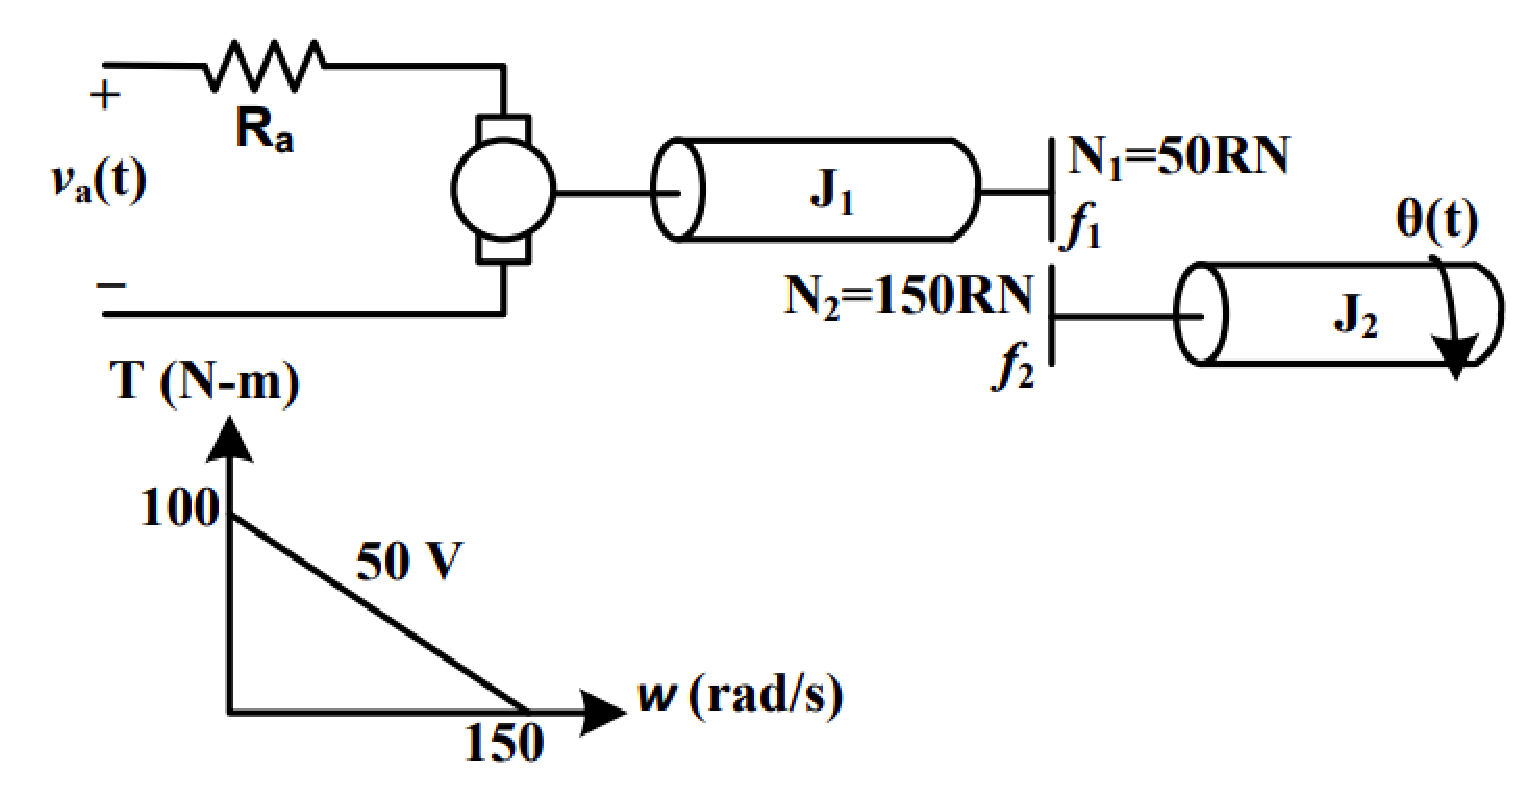
\includegraphics[width=\columnwidth]{./figs/ee18btech11001/ee18btech11001_1.eps}
  \caption{}
  \label{fig:ee18btech11001_fig1}
\end{figure}
%
\solution
Solving the system shown in \ref{fig:ee18btech11001_fig1},

From speed-torque curve of DC Motor in figure. Let $\vec{T_{m}}$ be the torque exerted by DC Motor.  \ref{fig:ee18btech11001_fig1}
\begin{align}
   \vec{T_{m}} &=  2V_{a} - \frac{2}{3}\bm{\omega_{1}}
    \label{eq:ee18btech11001_1}
\end{align}

\begin{table}[!ht]
\centering
%%%%%%%%%%%%%%%%%%%%%%%%%%%%%%%%%%%%%%%%%%%%%%%%%%%%%%%%%%%%%%%%%%%%%%
%%                                                                  %%
%%  This is the header of a LaTeX2e file exported from Gnumeric.    %%
%%                                                                  %%
%%  This file can be compiled as it stands or included in another   %%
%%  LaTeX document. The table is based on the longtable package so  %%
%%  the longtable options (headers, footers...) can be set in the   %%
%%  preamble section below (see PRAMBLE).                           %%
%%                                                                  %%
%%  To include the file in another, the following two lines must be %%
%%  in the including file:                                          %%
%%        \def\inputGnumericTable{}                                 %%
%%  at the beginning of the file and:                               %%
%%        \input{name-of-this-file.tex}                             %%
%%  where the table is to be placed. Note also that the including   %%
%%  file must use the following packages for the table to be        %%
%%  rendered correctly:                                             %%
%%    \usepackage[latin1]{inputenc}                                 %%
%%    \usepackage{color}                                            %%
%%    \usepackage{array}                                            %%
%%    \usepackage{longtable}                                        %%
%%    \usepackage{calc}                                             %%
%%    \usepackage{multirow}                                         %%
%%    \usepackage{hhline}                                           %%
%%    \usepackage{ifthen}                                           %%
%%  optionally (for landscape tables embedded in another document): %%
%%    \usepackage{lscape}                                           %%
%%                                                                  %%
%%%%%%%%%%%%%%%%%%%%%%%%%%%%%%%%%%%%%%%%%%%%%%%%%%%%%%%%%%%%%%%%%%%%%%



%%  This section checks if we are begin input into another file or  %%
%%  the file will be compiled alone. First use a macro taken from   %%
%%  the TeXbook ex 7.7 (suggestion of Han-Wen Nienhuys).            %%
\def\ifundefined#1{\expandafter\ifx\csname#1\endcsname\relax}


%%  Check for the \def token for inputed files. If it is not        %%
%%  defined, the file will be processed as a standalone and the     %%
%%  preamble will be used.                                          %%
\ifundefined{inputGnumericTable}

%%  We must be able to close or not the document at the end.        %%
	\def\gnumericTableEnd{\end{document}}


%%%%%%%%%%%%%%%%%%%%%%%%%%%%%%%%%%%%%%%%%%%%%%%%%%%%%%%%%%%%%%%%%%%%%%
%%                                                                  %%
%%  This is the PREAMBLE. Change these values to get the right      %%
%%  paper size and other niceties.                                  %%
%%                                                                  %%
%%%%%%%%%%%%%%%%%%%%%%%%%%%%%%%%%%%%%%%%%%%%%%%%%%%%%%%%%%%%%%%%%%%%%%

	\documentclass[12pt%
			  %,landscape%
                    ]{report}
       \usepackage[latin1]{inputenc}
       \usepackage{fullpage}
       \usepackage{color}
       \usepackage{array}
       \usepackage{longtable}
       \usepackage{calc}
       \usepackage{multirow}
       \usepackage{hhline}
       \usepackage{ifthen}

\begin{document}


%%  End of the preamble for the standalone. The next section is for %%
%%  documents which are included into other LaTeX2e files.          %%
\else

%%  We are not a stand alone document. For a regular table, we will %%
%%  have no preamble and only define the closing to mean nothing.   %%
    \def\gnumericTableEnd{}

%%  If we want landscape mode in an embedded document, comment out  %%
%%  the line above and uncomment the two below. The table will      %%
%%  begin on a new page and run in landscape mode.                  %%
%       \def\gnumericTableEnd{\end{landscape}}
%       \begin{landscape}


%%  End of the else clause for this file being \input.              %%
\fi

%%%%%%%%%%%%%%%%%%%%%%%%%%%%%%%%%%%%%%%%%%%%%%%%%%%%%%%%%%%%%%%%%%%%%%
%%                                                                  %%
%%  The rest is the gnumeric table, except for the closing          %%
%%  statement. Changes below will alter the table's appearance.     %%
%%                                                                  %%
%%%%%%%%%%%%%%%%%%%%%%%%%%%%%%%%%%%%%%%%%%%%%%%%%%%%%%%%%%%%%%%%%%%%%%

\providecommand{\gnumericmathit}[1]{#1} 
%%  Uncomment the next line if you would like your numbers to be in %%
%%  italics if they are italizised in the gnumeric table.           %%
%\renewcommand{\gnumericmathit}[1]{\mathit{#1}}
\providecommand{\gnumericPB}[1]%
{\let\gnumericTemp=\\#1\let\\=\gnumericTemp\hspace{0pt}}
 \ifundefined{gnumericTableWidthDefined}
        \newlength{\gnumericTableWidth}
        \newlength{\gnumericTableWidthComplete}
        \newlength{\gnumericMultiRowLength}
        \global\def\gnumericTableWidthDefined{}
 \fi
%% The following setting protects this code from babel shorthands.  %%
 \ifthenelse{\isundefined{\languageshorthands}}{}{\languageshorthands{english}}
%%  The default table format retains the relative column widths of  %%
%%  gnumeric. They can easily be changed to c, r or l. In that case %%
%%  you may want to comment out the next line and uncomment the one %%
%%  thereafter                                                      %%
\providecommand\gnumbox{\makebox[0pt]}
%%\providecommand\gnumbox[1][]{\makebox}

%% to adjust positions in multirow situations                       %%
\setlength{\bigstrutjot}{\jot}
\setlength{\extrarowheight}{\doublerulesep}

%%  The \setlongtables command keeps column widths the same across  %%
%%  pages. Simply comment out next line for varying column widths.  %%
\setlongtables

\setlength\gnumericTableWidth{%
	80pt+%
	50pt+%
	60pt+%
0pt}
\def\gumericNumCols{3}
\setlength\gnumericTableWidthComplete{\gnumericTableWidth+%
         \tabcolsep*\gumericNumCols*2+\arrayrulewidth*\gumericNumCols}
\ifthenelse{\lengthtest{\gnumericTableWidthComplete > \linewidth}}%
         {\def\gnumericScale{\ratio{\linewidth-%
                        \tabcolsep*\gumericNumCols*2-%
                        \arrayrulewidth*\gumericNumCols}%
{\gnumericTableWidth}}}%
{\def\gnumericScale{1}}

%%%%%%%%%%%%%%%%%%%%%%%%%%%%%%%%%%%%%%%%%%%%%%%%%%%%%%%%%%%%%%%%%%%%%%
%%                                                                  %%
%% The following are the widths of the various columns. We are      %%
%% defining them here because then they are easier to change.       %%
%% Depending on the cell formats we may use them more than once.    %%
%%                                                                  %%
%%%%%%%%%%%%%%%%%%%%%%%%%%%%%%%%%%%%%%%%%%%%%%%%%%%%%%%%%%%%%%%%%%%%%%

\ifthenelse{\isundefined{\gnumericColA}}{\newlength{\gnumericColA}}{}\settowidth{\gnumericColA}{\begin{tabular}{@{}p{30pt*\gnumericScale}@{}}x\end{tabular}}
\ifthenelse{\isundefined{\gnumericColC}}{\newlength{\gnumericColC}}{}\settowidth{\gnumericColC}{\begin{tabular}{@{}p{160pt*\gnumericScale}@{}}x\end{tabular}}
\begin{tabular}[c]{%
	b{\gnumericColA}%	
	b{\gnumericColC}%
	}

%%%%%%%%%%%%%%%%%%%%%%%%%%%%%%%%%%%%%%%%%%%%%%%%%%%%%%%%%%%%%%%%%%%%%%
%%  The longtable options. (Caption, headers... see Goosens, p.124) %%
%	\caption{The Table Caption.}             \\	%
% \hline	% Across the top of the table.
%%  The rest of these options are table rows which are placed on    %%
%%  the first, last or every page. Use \multicolumn if you want.    %%

%%  Header for the first page.                                      %%
%	\multicolumn{3}{c}{The First Header} \\ \hline 
%	\multicolumn{1}{c}{colTag}	%Column 1
%	&\multicolumn{1}{c}{colTag}	%Column 2
%	&\multicolumn{1}{c}{colTag}	\\ \hline %Last column
%	\endfirsthead

%%  The running header definition.                                  %%
%	\hline
%	\multicolumn{3}{l}{\ldots\small\slshape continued} \\ \hline
%	\multicolumn{1}{c}{colTag}	%Column 1
%	&\multicolumn{1}{c}{colTag}	%Column 2
%	&\multicolumn{1}{c}{colTag}	\\ \hline %Last column
%	\endhead

%%  The running footer definition.                                  %%
%	\hline
%	\multicolumn{3}{r}{\small\slshape continued\ldots} \\
%	\endfoot

%%  The ending footer definition.                                   %%
%	\multicolumn{3}{c}{That's all folks} \\ \hline 
%	\endlastfoot
%%%%%%%%%%%%%%%%%%%%%%%%%%%%%%%%%%%%%%%%%%%%%%%%%%%%%%%%%%%%%%%%%%%%%%


	
\hhline{|-|-}
	 \multicolumn{1}{|p{\gnumericColA}|}%
	{\gnumericPB{\centering}\textbf{Variable}}
	&\multicolumn{1}{p{\gnumericColC}|}%
	{\gnumericPB{\centering}\textbf{Description}}

\\

	

\hhline{|--|}
	 \multicolumn{1}{|p{\gnumericColA}|}%
	{\gnumericPB{\centering}$\Vec{T_{m}}$}
	&\multicolumn{1}{p{\gnumericColC}|}%
	{\gnumericPB{\centering}Torque applied by motor on left of $J_{1}$}
	
	
\\

	
	\hhline{|--|}
	 \multicolumn{1}{|p{\gnumericColA}|}%
	{\gnumericPB{\centering}$\Vec{T_{1}}$}
	&\multicolumn{1}{p{\gnumericColC}|}%
	{\gnumericPB{\centering}Torque existing on right of $J_{1}$}

\\

	\hhline{|--|}
	 \multicolumn{1}{|p{\gnumericColA}|}%
	{\gnumericPB{\centering}$\Vec{T_{2}}$}
	&\multicolumn{1}{p{\gnumericColC}|}%
	{\gnumericPB{\centering}Torque existing on left of $J_{2}$}

\\

	\hhline{|--|}
	 \multicolumn{1}{|p{\gnumericColA}|}%
	{\gnumericPB{\centering}$\bm{\theta_{1}}$}
	&\multicolumn{1}{p{\gnumericColC}|}%
	{\gnumericPB{\centering}Position vector of $J_{1}$}

\\

	\hhline{|--|}
	 \multicolumn{1}{|p{\gnumericColA}|}%
	{\gnumericPB{\centering}$\bm{\theta_{2}}$}
	&\multicolumn{1}{p{\gnumericColC}|}%
	{\gnumericPB{\centering}Position vector of $J_{2}$}

\\
	\hhline{|--|}
	 \multicolumn{1}{|p{\gnumericColA}|}%
	{\gnumericPB{\centering}$V_{a}$}
	&\multicolumn{1}{p{\gnumericColC}|}%
	{\gnumericPB{\centering}Armature voltage of DC Motor}

\\
	
	
	\hhline{|--|}
	 \multicolumn{1}{|p{\gnumericColA}|}%
	{\gnumericPB{\centering}$\bm{\omega_{1}}$}
	&\multicolumn{1}{p{\gnumericColC}|}%
	{\gnumericPB{\centering} Angular velocity of $J_{1}$}
\\
	\hhline{|--|}
	 \multicolumn{1}{|p{\gnumericColA}|}%
	{\gnumericPB{\centering}$J_{1}$}
	&\multicolumn{1}{p{\gnumericColC}|}%
	{\gnumericPB{\centering}Moment of Intertia of first load}

\\
	\hhline{|--|}
	 \multicolumn{1}{|p{\gnumericColA}|}%
	{\gnumericPB{\centering}$J_{2}$}
	&\multicolumn{1}{p{\gnumericColC}|}%
	{\gnumericPB{\centering}Moment of Intertia of second load}

\\
	\hhline{|--|}
	 \multicolumn{1}{|p{\gnumericColA}|}%
	{\gnumericPB{\centering}$f_{1}$}
	&\multicolumn{1}{p{\gnumericColC}|}%
	{\gnumericPB{\centering}Viscous friction on $J_{1}$}

\\
	\hhline{|--|}
	 \multicolumn{1}{|p{\gnumericColA}|}%
	{\gnumericPB{\centering}$f_{2}$}
	&\multicolumn{1}{p{\gnumericColC}|}%
	{\gnumericPB{\centering}Viscous friction on $J_{2}$}

\\

\hhline{|-|-}
\end{tabular}

\ifthenelse{\isundefined{\languageshorthands}}{}{\languageshorthands{\languagename}}
\gnumericTableEnd
\caption{List of Variables}
\label{table:ee18btech11001_3}
\end{table}
Change in torque across ends = torque applied on load + viscous friction. On $J_{1}$ at one end torque $T_{m}$ is applied and at the other end $T_{1}$ exists.
\begin{align}
    \vec{T_{m}} &= \vec{T_{1}} + J_{1}\bm{\Ddot{\theta_{1}}} + f_{1}\bm{\Dot{\theta_{1}}} 
    \label{eq:ee18btech11001_2}
\end{align}
Similarly for $J_{2}$
\begin{align}
    \vec{T_{2}} &=  J_{2}\bm{\Ddot{\theta_{2}}} + f_{2}\bm{\Dot{\theta_{2}}} 
    \label{eq:ee18btech11001_3}
    \\
    \vec{T_{2}} &= \frac{N_{2}}{N_{1}} \vec{T_{1}} \text{ (Gear Train Formula)} \label{eq:ee18btech11001_4}
    \\
    \bm{\theta_{2}} &= \frac{N_{1}}{N_{2}} \bm{\theta_{1}} \text{ (Gear Train Formula)} \label{eq:ee18btech11001_5}
\end{align}
    
Converting to State Space model
\begin{align}
    \bm{\theta} &= \myvec{\bm{\theta_{1}} \\ \bm{\theta_{2}}}
    \\
    3 \Vec{T_{m}} &= \myvec{3J_{1} & J_{2}}\bm{\Ddot{\theta}}+ \myvec{3f_{1} & f_{2}}\bm{\dot{\theta}}
    \\
    \Vec{T_{m}} &= 2V_{a} - \myvec{\frac{2}{3} & 0}\bm{\dot{\theta}}
    \\
    \bm{\theta} &= \myvec{N_{2} & N_{1}} K
\end{align}
On solving the above State Space Model
\begin{align}
    V_{a} &= 6\bm{\Ddot{\theta_{2}}} + 10\bm{\Dot{\theta_{2}}} \label{eq:ee18btech11001_6}
\end{align}
Taking Laplace transform
\begin{align}
   G(s) &=  K \frac{\theta (s)}{V_{a}(s)} = \frac{1}{2s(3s+5)} \label{eq:ee18btech11001_7}
\end{align}
From Error Constant  K = 500
\begin{align}
   G(s) &=  \frac{\theta (s)}{V_{a}(s)} = 250 \frac{1}{s(3s+5)} \label{eq:ee18btech11001_8}
   \\
   \zeta &= 0.0695
   \\
   M_{p} &= e^{\dfrac{-\zeta\pi}{\sqrt{1-\zeta^{2}}}} = 81.6\%
   \\
   \phi_{M} &= \tan^{-1}(\dfrac{2\zeta}{\sqrt{-2\zeta^2 + \sqrt{4\zeta^4 + 1}}})
   \\
   \phi_{max} &= 39.5\degree-7.35\degree+ \text{ correction factor}
   \\
   \phi_{max} &= 57\degree
\end{align}
\begin{table}[!ht]
\centering
%%%%%%%%%%%%%%%%%%%%%%%%%%%%%%%%%%%%%%%%%%%%%%%%%%%%%%%%%%%%%%%%%%%%%%
%%                                                                  %%
%%  This is the header of a LaTeX2e file exported from Gnumeric.    %%
%%                                                                  %%
%%  This file can be compiled as it stands or included in another   %%
%%  LaTeX document. The table is based on the longtable package so  %%
%%  the longtable options (headers, footers...) can be set in the   %%
%%  preamble section below (see PRAMBLE).                           %%
%%                                                                  %%
%%  To include the file in another, the following two lines must be %%
%%  in the including file:                                          %%
%%        \def\inputGnumericTable{}                                 %%
%%  at the beginning of the file and:                               %%
%%        \input{name-of-this-file.tex}                             %%
%%  where the table is to be placed. Note also that the including   %%
%%  file must use the following packages for the table to be        %%
%%  rendered correctly:                                             %%
%%    \usepackage[latin1]{inputenc}                                 %%
%%    \usepackage{color}                                            %%
%%    \usepackage{array}                                            %%
%%    \usepackage{longtable}                                        %%
%%    \usepackage{calc}                                             %%
%%    \usepackage{multirow}                                         %%
%%    \usepackage{hhline}                                           %%
%%    \usepackage{ifthen}                                           %%
%%  optionally (for landscape tables embedded in another document): %%
%%    \usepackage{lscape}                                           %%
%%                                                                  %%
%%%%%%%%%%%%%%%%%%%%%%%%%%%%%%%%%%%%%%%%%%%%%%%%%%%%%%%%%%%%%%%%%%%%%%



%%  This section checks if we are begin input into another file or  %%
%%  the file will be compiled alone. First use a macro taken from   %%
%%  the TeXbook ex 7.7 (suggestion of Han-Wen Nienhuys).            %%
\def\ifundefined#1{\expandafter\ifx\csname#1\endcsname\relax}


%%  Check for the \def token for inputed files. If it is not        %%
%%  defined, the file will be processed as a standalone and the     %%
%%  preamble will be used.                                          %%
\ifundefined{inputGnumericTable}

%%  We must be able to close or not the document at the end.        %%
	\def\gnumericTableEnd{\end{document}}


%%%%%%%%%%%%%%%%%%%%%%%%%%%%%%%%%%%%%%%%%%%%%%%%%%%%%%%%%%%%%%%%%%%%%%
%%                                                                  %%
%%  This is the PREAMBLE. Change these values to get the right      %%
%%  paper size and other niceties.                                  %%
%%                                                                  %%
%%%%%%%%%%%%%%%%%%%%%%%%%%%%%%%%%%%%%%%%%%%%%%%%%%%%%%%%%%%%%%%%%%%%%%

	\documentclass[12pt%
			  %,landscape%
                    ]{report}
       \usepackage[latin1]{inputenc}
       \usepackage{fullpage}
       \usepackage{color}
       \usepackage{array}
       \usepackage{longtable}
       \usepackage{calc}
       \usepackage{multirow}
       \usepackage{hhline}
       \usepackage{ifthen}

\begin{document}


%%  End of the preamble for the standalone. The next section is for %%
%%  documents which are included into other LaTeX2e files.          %%
\else

%%  We are not a stand alone document. For a regular table, we will %%
%%  have no preamble and only define the closing to mean nothing.   %%
    \def\gnumericTableEnd{}

%%  If we want landscape mode in an embedded document, comment out  %%
%%  the line above and uncomment the two below. The table will      %%
%%  begin on a new page and run in landscape mode.                  %%
%       \def\gnumericTableEnd{\end{landscape}}
%       \begin{landscape}


%%  End of the else clause for this file being \input.              %%
\fi

%%%%%%%%%%%%%%%%%%%%%%%%%%%%%%%%%%%%%%%%%%%%%%%%%%%%%%%%%%%%%%%%%%%%%%
%%                                                                  %%
%%  The rest is the gnumeric table, except for the closing          %%
%%  statement. Changes below will alter the table's appearance.     %%
%%                                                                  %%
%%%%%%%%%%%%%%%%%%%%%%%%%%%%%%%%%%%%%%%%%%%%%%%%%%%%%%%%%%%%%%%%%%%%%%

\providecommand{\gnumericmathit}[1]{#1} 
%%  Uncomment the next line if you would like your numbers to be in %%
%%  italics if they are italizised in the gnumeric table.           %%
%\renewcommand{\gnumericmathit}[1]{\mathit{#1}}
\providecommand{\gnumericPB}[1]%
{\let\gnumericTemp=\\#1\let\\=\gnumericTemp\hspace{0pt}}
 \ifundefined{gnumericTableWidthDefined}
        \newlength{\gnumericTableWidth}
        \newlength{\gnumericTableWidthComplete}
        \newlength{\gnumericMultiRowLength}
        \global\def\gnumericTableWidthDefined{}
 \fi
%% The following setting protects this code from babel shorthands.  %%
 \ifthenelse{\isundefined{\languageshorthands}}{}{\languageshorthands{english}}
%%  The default table format retains the relative column widths of  %%
%%  gnumeric. They can easily be changed to c, r or l. In that case %%
%%  you may want to comment out the next line and uncomment the one %%
%%  thereafter                                                      %%
\providecommand\gnumbox{\makebox[0pt]}
%%\providecommand\gnumbox[1][]{\makebox}

%% to adjust positions in multirow situations                       %%
\setlength{\bigstrutjot}{\jot}
\setlength{\extrarowheight}{\doublerulesep}

%%  The \setlongtables command keeps column widths the same across  %%
%%  pages. Simply comment out next line for varying column widths.  %%
\setlongtables

\setlength\gnumericTableWidth{%
	80pt+%
	50pt+%
	60pt+%
0pt}
\def\gumericNumCols{3}
\setlength\gnumericTableWidthComplete{\gnumericTableWidth+%
         \tabcolsep*\gumericNumCols*2+\arrayrulewidth*\gumericNumCols}
\ifthenelse{\lengthtest{\gnumericTableWidthComplete > \linewidth}}%
         {\def\gnumericScale{\ratio{\linewidth-%
                        \tabcolsep*\gumericNumCols*2-%
                        \arrayrulewidth*\gumericNumCols}%
{\gnumericTableWidth}}}%
{\def\gnumericScale{1}}

%%%%%%%%%%%%%%%%%%%%%%%%%%%%%%%%%%%%%%%%%%%%%%%%%%%%%%%%%%%%%%%%%%%%%%
%%                                                                  %%
%% The following are the widths of the various columns. We are      %%
%% defining them here because then they are easier to change.       %%
%% Depending on the cell formats we may use them more than once.    %%
%%                                                                  %%
%%%%%%%%%%%%%%%%%%%%%%%%%%%%%%%%%%%%%%%%%%%%%%%%%%%%%%%%%%%%%%%%%%%%%%

\ifthenelse{\isundefined{\gnumericColA}}{\newlength{\gnumericColA}}{}\settowidth{\gnumericColA}{\begin{tabular}{@{}p{80pt*\gnumericScale}@{}}x\end{tabular}}

\ifthenelse{\isundefined{\gnumericColB}}{\newlength{\gnumericColB}}{}\settowidth{\gnumericColB}{\begin{tabular}{@{}p{50pt*\gnumericScale}@{}}x\end{tabular}}

\ifthenelse{\isundefined{\gnumericColC}}{\newlength{\gnumericColC}}{}\settowidth{\gnumericColC}{\begin{tabular}{@{}p{60pt*\gnumericScale}@{}}x\end{tabular}}
\begin{tabular}[c]{%
	b{\gnumericColA}%	
	b{\gnumericColB}%
	b{\gnumericColC}%
	}

%%%%%%%%%%%%%%%%%%%%%%%%%%%%%%%%%%%%%%%%%%%%%%%%%%%%%%%%%%%%%%%%%%%%%%
%%  The longtable options. (Caption, headers... see Goosens, p.124) %%
%	\caption{The Table Caption.}             \\	%
% \hline	% Across the top of the table.
%%  The rest of these options are table rows which are placed on    %%
%%  the first, last or every page. Use \multicolumn if you want.    %%

%%  Header for the first page.                                      %%
%	\multicolumn{3}{c}{The First Header} \\ \hline 
%	\multicolumn{1}{c}{colTag}	%Column 1
%	&\multicolumn{1}{c}{colTag}	%Column 2
%	&\multicolumn{1}{c}{colTag}	\\ \hline %Last column
%	\endfirsthead

%%  The running header definition.                                  %%
%	\hline
%	\multicolumn{3}{l}{\ldots\small\slshape continued} \\ \hline
%	\multicolumn{1}{c}{colTag}	%Column 1
%	&\multicolumn{1}{c}{colTag}	%Column 2
%	&\multicolumn{1}{c}{colTag}	\\ \hline %Last column
%	\endhead

%%  The running footer definition.                                  %%
%	\hline
%	\multicolumn{3}{r}{\small\slshape continued\ldots} \\
%	\endfoot

%%  The ending footer definition.                                   %%
%	\multicolumn{3}{c}{That's all folks} \\ \hline 
%	\endlastfoot
%%%%%%%%%%%%%%%%%%%%%%%%%%%%%%%%%%%%%%%%%%%%%%%%%%%%%%%%%%%%%%%%%%%%%%


	
\hhline{|-|-|-}
	 \multicolumn{1}{|p{\gnumericColA}|}%
	{\gnumericPB{\centering}\textbf{Specifications}}
	&\multicolumn{1}{p{\gnumericColB}|}%
	{\gnumericPB{\centering}\textbf{Actual}}
	&\multicolumn{1}{p{\gnumericColC}|}%
	{\gnumericPB{\centering}\textbf{Expected}}

\\

	

\hhline{|---|}
	 \multicolumn{1}{|p{\gnumericColA}|}%
	{\gnumericPB{\centering}OS\%}
	&\multicolumn{1}{p{\gnumericColB}|}%
	{\gnumericPB{\centering}81.6\%}
	&\multicolumn{1}{p{\gnumericColC}|}%
	{\gnumericPB{\centering}25\%}
	
	
\\

	
	\hhline{|---|}
	 \multicolumn{1}{|p{\gnumericColA}|}%
	{\gnumericPB{\centering}$\zeta$}
	&\multicolumn{1}{p{\gnumericColB}|}%
	{\gnumericPB{\centering}0.0695}
	&\multicolumn{1}{p{\gnumericColC}|}%
	{\gnumericPB{\centering}0.403}

\\

	
	
	\hhline{|---|}
	 \multicolumn{1}{|p{\gnumericColA}|}%
	{\gnumericPB{\centering}$\phi_{m}$}
	&\multicolumn{1}{p{\gnumericColB}|}%
	{\gnumericPB{\centering}$7.35^\circ$}
	&\multicolumn{1}{p{\gnumericColC}|}%
	{\gnumericPB{\centering}$39.5^ \circ$ }
\\

\hhline{|-|-|-}
\end{tabular}

\ifthenelse{\isundefined{\languageshorthands}}{}{\languageshorthands{\languagename}}
\gnumericTableEnd
\caption{Table of Specifications}
\label{table:ee18btech11001}
\end{table}

\textbf{Designing a lead compensator}
\begin{align}
   G_{c}(s) &=  \frac{1}{a}\frac{s + \frac{1}{T}}{s + \frac{1}{aT}} (a<1) \label{eq:ee18btech11001_9}
   \\
   \sin\phi_{max} &= \dfrac{a-1}{a+1}
   \\
   a &= 0.1
\end{align}
\begin{align}
   |G(j\omega_{c})| &= \frac{1}{\sqrt{a}} = 10 dB
   \\
   \omega_{c} &= 5\degree \text{  (Refer figure \ref{fig:ee18btech11001_fig3})}
   \\
   T &= \frac{1}{\omega_{c}\sqrt{a}} = 0.632
   \\
   G_{c}(s) &=  10 \frac{s + 1.6}{s + 16}
   \\
   G(s)G_{c}(s)  &= 2500 \dfrac{s+1.6}{s(3s+5)(s+16)} \label{eq:ee18btech11001_10}
\end{align}

\textbf{Designing a lag compensator}
\begin{align}
   G_{c}(s) &=  \frac{1}{b}\frac{s + \frac{1}{T}}{s + \frac{1}{bT}} (b>1)  \label{eq:ee18btech11001_11}
   \\
   \phi_{max}  &= 39.5\degree -7.35\degree + correction factor
   \\
   \phi_{max} &= 45 \degree
\end{align}
\begin{figure}[!ht]
\centering
    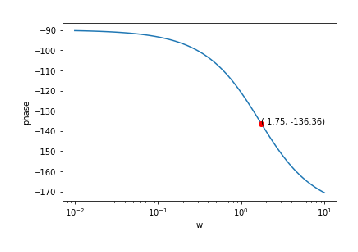
\includegraphics[width=\columnwidth]{./figs/ee18btech11001/ee18btech11001_3.eps}
  \caption{Phase plot of G(s)}
  \label{fig:ee18btech11001_fig2}
\end{figure}

$\omega_{c} = $ Frequency at which phase of bode plot of G(s) is -180 $+ \phi_{max}$ i.e. -135 \degree

$\omega_{c}  = 1.75 rad/sec$  as in Figure \ref{fig:ee18btech11001_fig2}

We place the zero at 
\begin{align} 
   \omega &= 0.2\omega_{c} = 0.35 rad/sec 
   \\
   \implies T &= 2.85
\end{align}
\begin{figure}[!ht]
\centering
    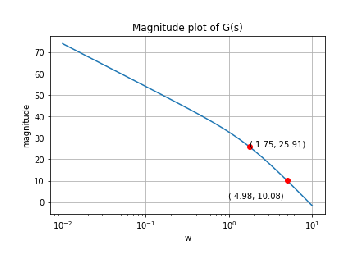
\includegraphics[width=\columnwidth]{./figs/ee18btech11001/ee18btech11001_2.eps}
  \caption{Magnitude plot of G(s)}
  \label{fig:ee18btech11001_fig3}
\end{figure}
\begin{lstlisting}
codes/ee18btech11001/ee18btech11001_1.py
\end{lstlisting}

The magnitude of $G(j\omega)$ at the new gain crossover frequency  $\omega_{c} = 1.75 rad/sec$ is 26 dB as in figure \ref{fig:ee18btech11001_fig3}.In order to have $\omega_{c}$  as the new gain crossover frequency, the lag compensator
must give an attenuation of -26db at $\omega_{c}$
\begin{align}
    -20 \log{b} &= -26dB
    \\
    b &= 19.95 \approx 20
    \\
    G_{c}(s) &=  0.05\frac{s + 0.35}{s + 0.0175}
    \\
    G(s)G_{c}(s) &= 12.5 \dfrac{s+0.35}{s(3s+5)(s+0.0175)} \label{eq:ee18btech11001_12}
\end{align}


\textbf{Performance Evaluation of compensators}

The following code plots the performance curves

\begin{lstlisting}[frame=single]
codes/ee18btech11001/ee18btech11001_2.py
\end{lstlisting}
\begin{figure}[!ht]
\centering
    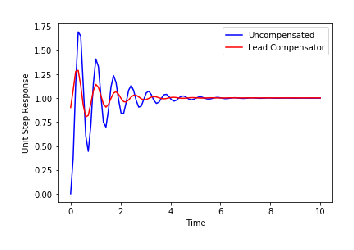
\includegraphics[width=\columnwidth]{./figs/ee18btech11001/ee18btech11001_4.eps}
  \caption{Performance of Lead Compensator}
  \label{fig:ee18btech11001_fig4}
\end{figure}
\begin{figure}[!ht]
\centering
    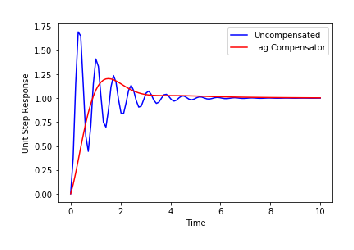
\includegraphics[width=\columnwidth]{./figs/ee18btech11001/ee18btech11001_5.eps}
  \caption{Performance of Lag Compensator}
  \label{fig:ee18btech11001_fig5}
\end{figure}

\begin{table}[!ht]
\centering
%%%%%%%%%%%%%%%%%%%%%%%%%%%%%%%%%%%%%%%%%%%%%%%%%%%%%%%%%%%%%%%%%%%%%%
%%                                                                  %%
%%  This is the header of a LaTeX2e file exported from Gnumeric.    %%
%%                                                                  %%
%%  This file can be compiled as it stands or included in another   %%
%%  LaTeX document. The table is based on the longtable package so  %%
%%  the longtable options (headers, footers...) can be set in the   %%
%%  preamble section below (see PRAMBLE).                           %%
%%                                                                  %%
%%  To include the file in another, the following two lines must be %%
%%  in the including file:                                          %%
%%        \def\inputGnumericTable{}                                 %%
%%  at the beginning of the file and:                               %%
%%        \input{name-of-this-file.tex}                             %%
%%  where the table is to be placed. Note also that the including   %%
%%  file must use the following packages for the table to be        %%
%%  rendered correctly:                                             %%
%%    \usepackage[latin1]{inputenc}                                 %%
%%    \usepackage{color}                                            %%
%%    \usepackage{array}                                            %%
%%    \usepackage{longtable}                                        %%
%%    \usepackage{calc}                                             %%
%%    \usepackage{multirow}                                         %%
%%    \usepackage{hhline}                                           %%
%%    \usepackage{ifthen}                                           %%
%%  optionally (for landscape tables embedded in another document): %%
%%    \usepackage{lscape}                                           %%
%%                                                                  %%
%%%%%%%%%%%%%%%%%%%%%%%%%%%%%%%%%%%%%%%%%%%%%%%%%%%%%%%%%%%%%%%%%%%%%%



%%  This section checks if we are begin input into another file or  %%
%%  the file will be compiled alone. First use a macro taken from   %%
%%  the TeXbook ex 7.7 (suggestion of Han-Wen Nienhuys).            %%
\def\ifundefined#1{\expandafter\ifx\csname#1\endcsname\relax}


%%  Check for the \def token for inputed files. If it is not        %%
%%  defined, the file will be processed as a standalone and the     %%
%%  preamble will be used.                                          %%
\ifundefined{inputGnumericTable}

%%  We must be able to close or not the document at the end.        %%
	\def\gnumericTableEnd{\end{document}}


%%%%%%%%%%%%%%%%%%%%%%%%%%%%%%%%%%%%%%%%%%%%%%%%%%%%%%%%%%%%%%%%%%%%%%
%%                                                                  %%
%%  This is the PREAMBLE. Change these values to get the right      %%
%%  paper size and other niceties.                                  %%
%%                                                                  %%
%%%%%%%%%%%%%%%%%%%%%%%%%%%%%%%%%%%%%%%%%%%%%%%%%%%%%%%%%%%%%%%%%%%%%%

	\documentclass[12pt%
			  %,landscape%
                    ]{report}
       \usepackage[latin1]{inputenc}
       \usepackage{fullpage}
       \usepackage{color}
       \usepackage{array}
       \usepackage{longtable}
       \usepackage{calc}
       \usepackage{multirow}
       \usepackage{hhline}
       \usepackage{ifthen}

\begin{document}


%%  End of the preamble for the standalone. The next section is for %%
%%  documents which are included into other LaTeX2e files.          %%
\else

%%  We are not a stand alone document. For a regular table, we will %%
%%  have no preamble and only define the closing to mean nothing.   %%
    \def\gnumericTableEnd{}

%%  If we want landscape mode in an embedded document, comment out  %%
%%  the line above and uncomment the two below. The table will      %%
%%  begin on a new page and run in landscape mode.                  %%
%       \def\gnumericTableEnd{\end{landscape}}
%       \begin{landscape}


%%  End of the else clause for this file being \input.              %%
\fi

%%%%%%%%%%%%%%%%%%%%%%%%%%%%%%%%%%%%%%%%%%%%%%%%%%%%%%%%%%%%%%%%%%%%%%
%%                                                                  %%
%%  The rest is the gnumeric table, except for the closing          %%
%%  statement. Changes below will alter the table's appearance.     %%
%%                                                                  %%
%%%%%%%%%%%%%%%%%%%%%%%%%%%%%%%%%%%%%%%%%%%%%%%%%%%%%%%%%%%%%%%%%%%%%%

\providecommand{\gnumericmathit}[1]{#1} 
%%  Uncomment the next line if you would like your numbers to be in %%
%%  italics if they are italizised in the gnumeric table.           %%
%\renewcommand{\gnumericmathit}[1]{\mathit{#1}}
\providecommand{\gnumericPB}[1]%
{\let\gnumericTemp=\\#1\let\\=\gnumericTemp\hspace{0pt}}
 \ifundefined{gnumericTableWidthDefined}
        \newlength{\gnumericTableWidth}
        \newlength{\gnumericTableWidthComplete}
        \newlength{\gnumericMultiRowLength}
        \global\def\gnumericTableWidthDefined{}
 \fi
%% The following setting protects this code from babel shorthands.  %%
 \ifthenelse{\isundefined{\languageshorthands}}{}{\languageshorthands{english}}
%%  The default table format retains the relative column widths of  %%
%%  gnumeric. They can easily be changed to c, r or l. In that case %%
%%  you may want to comment out the next line and uncomment the one %%
%%  thereafter                                                      %%
\providecommand\gnumbox{\makebox[0pt]}
%%\providecommand\gnumbox[1][]{\makebox}

%% to adjust positions in multirow situations                       %%
\setlength{\bigstrutjot}{\jot}
\setlength{\extrarowheight}{\doublerulesep}

%%  The \setlongtables command keeps column widths the same across  %%
%%  pages. Simply comment out next line for varying column widths.  %%
\setlongtables

\setlength\gnumericTableWidth{%
	80pt+%
	50pt+%
	60pt+%
0pt}
\def\gumericNumCols{3}
\setlength\gnumericTableWidthComplete{\gnumericTableWidth+%
         \tabcolsep*\gumericNumCols*2+\arrayrulewidth*\gumericNumCols}
\ifthenelse{\lengthtest{\gnumericTableWidthComplete > \linewidth}}%
         {\def\gnumericScale{\ratio{\linewidth-%
                        \tabcolsep*\gumericNumCols*2-%
                        \arrayrulewidth*\gumericNumCols}%
{\gnumericTableWidth}}}%
{\def\gnumericScale{1}}

%%%%%%%%%%%%%%%%%%%%%%%%%%%%%%%%%%%%%%%%%%%%%%%%%%%%%%%%%%%%%%%%%%%%%%
%%                                                                  %%
%% The following are the widths of the various columns. We are      %%
%% defining them here because then they are easier to change.       %%
%% Depending on the cell formats we may use them more than once.    %%
%%                                                                  %%
%%%%%%%%%%%%%%%%%%%%%%%%%%%%%%%%%%%%%%%%%%%%%%%%%%%%%%%%%%%%%%%%%%%%%%

\ifthenelse{\isundefined{\gnumericColA}}{\newlength{\gnumericColA}}{}\settowidth{\gnumericColA}{\begin{tabular}{@{}p{80pt*\gnumericScale}@{}}x\end{tabular}}

\ifthenelse{\isundefined{\gnumericColB}}{\newlength{\gnumericColB}}{}\settowidth{\gnumericColB}{\begin{tabular}{@{}p{50pt*\gnumericScale}@{}}x\end{tabular}}

\ifthenelse{\isundefined{\gnumericColC}}{\newlength{\gnumericColC}}{}\settowidth{\gnumericColC}{\begin{tabular}{@{}p{60pt*\gnumericScale}@{}}x\end{tabular}}
\begin{tabular}[c]{%
	b{\gnumericColA}%	
	b{\gnumericColB}%
	b{\gnumericColC}%
	}

%%%%%%%%%%%%%%%%%%%%%%%%%%%%%%%%%%%%%%%%%%%%%%%%%%%%%%%%%%%%%%%%%%%%%%
%%  The longtable options. (Caption, headers... see Goosens, p.124) %%
%	\caption{The Table Caption.}             \\	%
% \hline	% Across the top of the table.
%%  The rest of these options are table rows which are placed on    %%
%%  the first, last or every page. Use \multicolumn if you want.    %%

%%  Header for the first page.                                      %%
%	\multicolumn{3}{c}{The First Header} \\ \hline 
%	\multicolumn{1}{c}{colTag}	%Column 1
%	&\multicolumn{1}{c}{colTag}	%Column 2
%	&\multicolumn{1}{c}{colTag}	\\ \hline %Last column
%	\endfirsthead

%%  The running header definition.                                  %%
%	\hline
%	\multicolumn{3}{l}{\ldots\small\slshape continued} \\ \hline
%	\multicolumn{1}{c}{colTag}	%Column 1
%	&\multicolumn{1}{c}{colTag}	%Column 2
%	&\multicolumn{1}{c}{colTag}	\\ \hline %Last column
%	\endhead

%%  The running footer definition.                                  %%
%	\hline
%	\multicolumn{3}{r}{\small\slshape continued\ldots} \\
%	\endfoot

%%  The ending footer definition.                                   %%
%	\multicolumn{3}{c}{That's all folks} \\ \hline 
%	\endlastfoot
%%%%%%%%%%%%%%%%%%%%%%%%%%%%%%%%%%%%%%%%%%%%%%%%%%%%%%%%%%%%%%%%%%%%%%


	
\hhline{|-|-|-}
	 \multicolumn{1}{|p{\gnumericColA}|}%
	{\gnumericPB{\centering}\textbf{Compensator}}
	&\multicolumn{1}{p{\gnumericColB}|}%
	{\gnumericPB{\centering}\textbf{Actual OS\%}}
	&\multicolumn{1}{p{\gnumericColC}|}%
	{\gnumericPB{\centering}\textbf{Expected OS\%}}

\\

	

\hhline{|---|}
	 \multicolumn{1}{|p{\gnumericColA}|}%
	{\gnumericPB{\centering}Lead Compensator}
	&\multicolumn{1}{p{\gnumericColB}|}%
	{\gnumericPB{\centering}26\%}
	&\multicolumn{1}{p{\gnumericColC}|}%
	{\gnumericPB{\centering}25\%}
	
	
\\

	
	\hhline{|---|}
	 \multicolumn{1}{|p{\gnumericColA}|}%
	{\gnumericPB{\centering}Lag Compensator}
	&\multicolumn{1}{p{\gnumericColB}|}%
	{\gnumericPB{\centering}25\%}
	&\multicolumn{1}{p{\gnumericColC}|}%
	{\gnumericPB{\centering}24\%}

\\

\hhline{|-|-|-}
\end{tabular}

\ifthenelse{\isundefined{\languageshorthands}}{}{\languageshorthands{\languagename}}
\gnumericTableEnd
\caption{Performance comparison}
\label{table:ee18btech11001_2}
\end{table}
Figures \ref{fig:ee18btech11001_fig4} and \ref{fig:ee18btech11001_fig5} show the reduced overshoot \& settling time for unit step input. 

This verifies that the designed lead and lag compensators work as per specifications. 
%\end{enumerate}